\documentclass{beamer}
\usepackage[german]{babel}
%\usepackage{libertine}
%\renewcommand*\familydefault{\sfdefault}  %%
\usepackage[default]{opensans}
%\usepackage{gillius2}
%\usepackage{lato}
\usepackage{siunitx}

\usepackage[utf8]{inputenc}

\usepackage[T1]{fontenc}

\usepackage{booktabs} % To thicken table lines
\usepackage{multirow}


\usepackage{microtype}
\usepackage{xcolor,multido,colortbl}
\usepackage{pgffor}

\usepackage{tikz}
\usepackage[version=4]{mhchem}
\usepackage{tikzorbital}

\usepackage{pgfplots}
\pgfplotsset{compat=1.13} 
 %\pgfplotsset{com  =1.13}
\usepackage{graphicx}
\usepackage{adjustbox}
\usepackage{hyperref}
\usepackage{caption}

\usepgfmodule{matrix} 
\usetikzlibrary{matrix,positioning}
\usetikzlibrary{arrows}
\usetikzlibrary{calc,shapes}
\usetikzlibrary{backgrounds}
\newcommand{\makemycolor}[2]{%
    \pgfmathsetmacro{\hue}{(#1/100)^1.715*0.79}%
    \definecolor{myhsbcolor}{hsb}{\hue,1,1}%
    \textcolor{myhsbcolor}{#2}%
}

\usepackage[absolute,overlay]{textpos}




\tikzset{
    level1/.style = {
        ultra thick,
        green
    },
    level4/.style = {
        ultra thick,
        blue
    },
    level5/.style = {
        ultra thick,
        red
    }
}

\newcommand\ytl[2]{
\parbox[b]{8em}{\hfill{\color{cyan}\bfseries\sffamily #1}~$\cdots\cdots$~}\makebox[0pt][c]{$\bullet$}\vrule\quad \parbox[c]{4.5cm}{\vspace{7pt}\color{red!40!black!80}\raggedright\sffamily #2.\\[7pt]}\\[-3pt]}
%\usepackage[texcoord,grid,gridunit=mm,gridcolor=red!10,subgridcolor=green!10]{eso-pic}
\setbeamertemplate{navigation symbols}{}


\title{Lumineszenz von Seltenerd-Ionen}
\author{Nevroz Arslan}

\begin{document}
  {%
    \setbeamertemplate{headline}{}
   \setbeamercolor{postit}{fg=black,bg=yellow}
    \frame{\titlepage}
  }

    
\begin{frame}[t]\frametitle{Leuchtstoffe und AnwendungsBereiche}
    

    \begin{tabular}{lccccc}
\toprule
\multirow{2}{*}{Leuchtstoff}& Abk. &  \ce{$\lambda$} & Abs. bei  & QE & LE  \\
& &\si{\nano\meter}&254 \si{\nano\meter}  & \% & \si{\lumen\per\watt}\\
\midrule
 \ce{BaMgAl_{10}O_{17}:Eu}& BAM & \cellcolor[wave]{450} 450  & 90 &  90 &90\\
\ce{(Ce,Tb)MgAl_{11}O_{19}}   & CAT   &  \cellcolor[wave]{542} 542  &  95 & 90& 495\\
\ce{Y_2O_3:Eu}    & YOX   &  \cellcolor[wave]{611} 611  &  75 & 90 &280\\
 \ce{BaMgAl_{10}O_{17}:Eu}  & BAM-Mn  & \cellcolor[wave]{520} 520 &  & & \\
\ce{MgGePO_{5.5}F:Mn}  & MGM  & \cellcolor[wave]{655} 655 & 95 &80 & 80\\
\ce{Sr_2P_2O_7:Eu}  & SPE  & \cellcolor[wave]{420} 420 &  & & \\
\bottomrule
\end{tabular}

\begin{figure}[!h]
\centering
      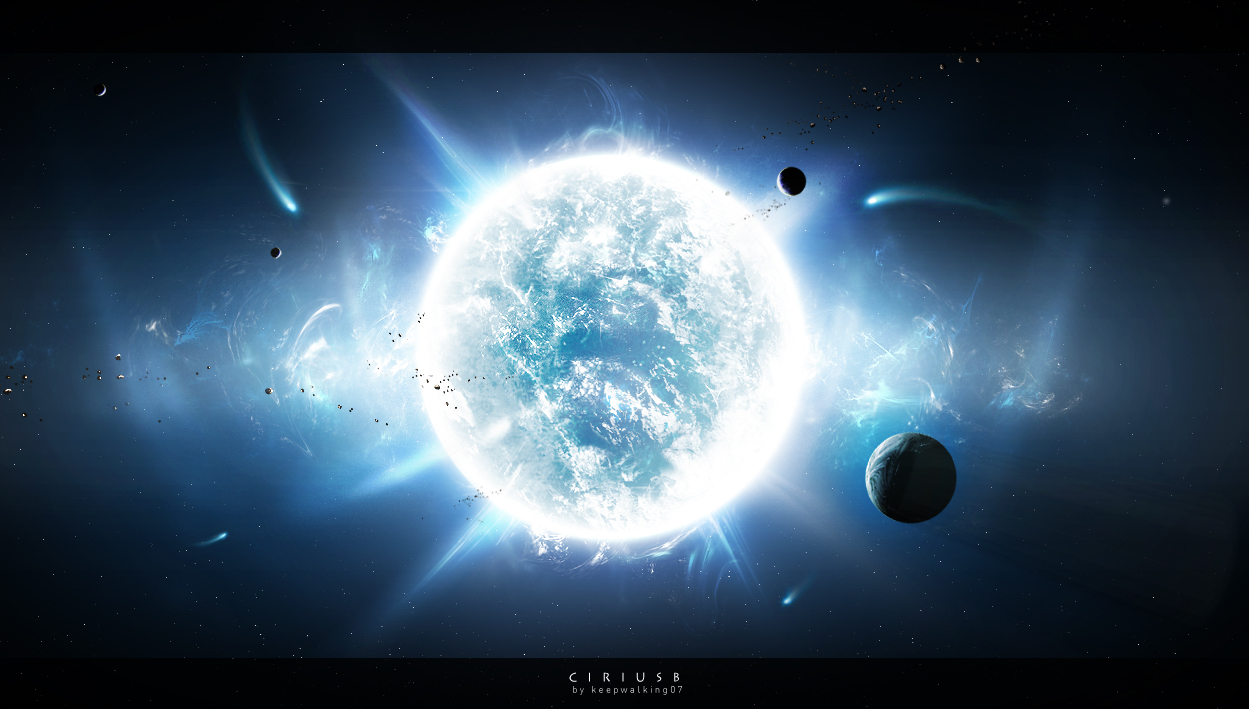
\includegraphics[scale=0.3]{siriusb.jpg}
      \caption*{\footnotesize Handelsübliche Leuchtstoffe}
 \end{figure}
\end{frame}

\begin{frame}[t]\frametitle{Lumineszenz}
    
\begin{figure}[!h]
\centering
      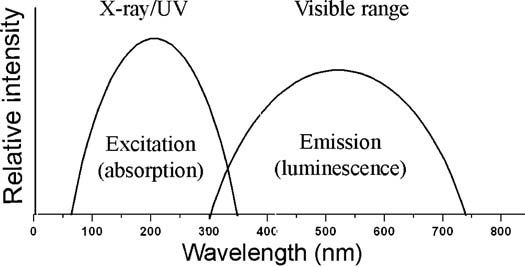
\includegraphics[scale=0.3]{stokes.jpg}
      \caption*{\footnotesize Stokes Verschiebung }
 \end{figure}

\end{frame}





\begin{frame}[t]\frametitle{Scheelite \ce{CaWO4} als Wirtgitter}
     \begin{columns}
      \column{.5\textwidth}
              \begin{figure}[!h]
\centering
      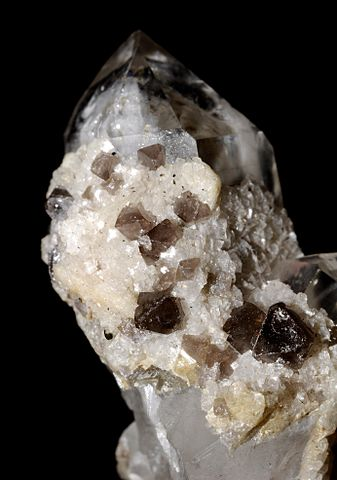
\includegraphics{scheelitesurquarz.jpg}
      \caption*{\footnotesize Scheelite ist ein häufig vorkommendes Mineral}
 \end{figure}
  \column{.5\textwidth}
  
 \begin{figure}[!h]
\centering
      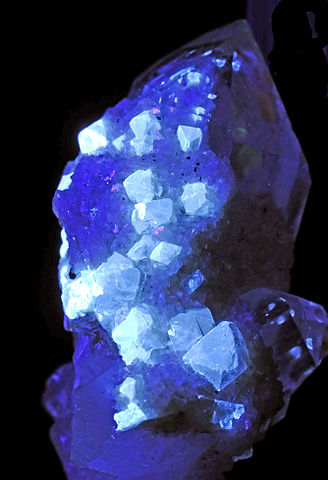
\includegraphics{scheelitesurquarz2.jpg}
     
      \caption*{\footnotesize \ce{CaWO_4} unter UV-Licht}
 \end{figure}
      \end{columns}

 \begin{itemize}
      \item \footnotesize ein geringer Zusatz an Samarium verändert die Farbe ins gelborange.
    \end{itemize}   

\end{frame}


\begin{frame}[t]\frametitle{Konzentrations abhängigkeit der Emmision}
 \begin{columns}
    \column{.6\textwidth}
    \begin{itemize}
      \item \footnotesize rote Emmision \ce{Eu^{3+}} erst bei Konzentration 2.5 \% \si{\mol} 
      \item  \footnotesize hypersensitive electric dipole transition  \ce{5D_1 -> 7F_2}
    \end{itemize}
     \column{.4\textwidth}
      \begin{figure}[!h]
\centering
     \begin{tikzpicture}
\node[inner sep=0pt] (russell) at (0,0)
    {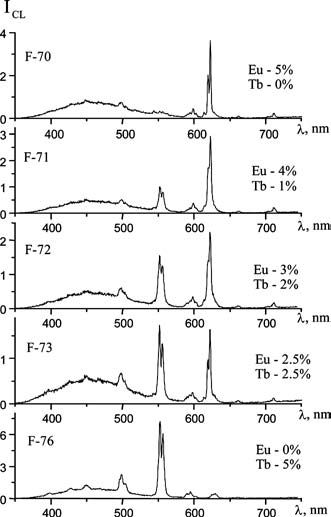
\includegraphics[scale=0.35]{scheelite.jpg}};
     \colorlet{color min hsb}[hsb]{red}
  \colorlet{color max hsb}[hsb]{violet}
   \foreach \pos in {100,...,0}{
    \colorlet{my color hsb}[rgb]{color min hsb!\pos!color max hsb}
    \fill[fill=my color hsb,draw=none] (-1.7+\pos/36,-3.4) rectangle +(5mm,1mm);
  }
\end{tikzpicture}

      \caption*{\tiny \ce{CaWO4:Eu^{3+}, Tb^{3+} }}
 \end{figure}
 \end{columns}

\end{frame}
%http://www.rsc.org/chemistryworld/News/2009/September/01090901.asp
%https://www.osapublishing.org/oe/fulltext.cfm?uri=oe-19-S3-A331
\end{document}

% Reference